\section{Implementation}

\paragraph{}
This section describes the implementation of the project's software.

\subsection{Platform}

\paragraph{}
This section covers all concrete choices made regarding third-party software libraries and systems in addition to any third-party project infrastructure included in the project.

\subsubsection{Bootloader}

\paragraph{}
The bootloader chosen for this project is Das U-Boot \cite{uboot}, an open source bootloader supporting several embedded architectures.
This software exposes all the necessary facilities to locate, load and execute the real operating system kernel which will host the project's software.

\subsubsection{Operating System}

\paragraph{}
The operating system chosen for this project is Linux, an open source operating system kernel that runs on many embedded computer systems as well as larger ones \cite{linux-readme}.
Much of the software written for this project will run on any UNIX-like operating system, however.

\subsubsection{Frameworks}

\paragraph{}
When developing applications, the choice of frameworks can be the most significant driving influence in the implementations of a project.
While this project has chosen Linux as its operating system, it has been developed heavily with portable libraries that can be built (and run) on other operating systems and architectures.
This project has chosen to only build upon open source libraries.

\paragraph{}
At the lowest level, all the application code of this project uses GLib \cite{glib-overview}, a portable utility library providing many data structures and support functionality to assist application development.
GLib also includes GObject, a C-based object-oriented type system, and GIO, an asynchronous Input/Output (I/O) library with many more additional application support features.
Importantly, GIO provides a client and server implementation of the D-Bus protocol using GIO's asynchronous I/O model.

\subsubsection{Programming Language}

\paragraph{}
Initially, this project was programmed in Vala, a language with a similar syntactical appearance to C\# but targeting the GObject type system.
This is achieved by the Vala compiler generating GObject-style C code and mapping documentation annotations as well as custom metadata to Vala constructs.
Since Vala is just a code generator, its use does not require a virtual machine, runtime interpreter, or garbage collector.
These properties are advantageous to embedded software development where processing speed, memory usage, and power consumption are less abundant than desktop or server environments.
Vala allows for fairly rapid prototype development due to its significantly smaller amount of boilerplate code necessary to define and implement object-oriented constructs such as interfaces and classes (as well as subclassing).
Through the development of the project, many difficulties were experienced with this language that required the author to fix bugs within the Vala language or its bindings to external libraries.
Furthermore, the nature of the Vala language and libraries implemented with the GObject type system introduce a maintenance requirement for the Vala bindings to a specific library.
Changes to APIs and incorrect transcription or scanning will lead to discrepancies between the original C API of a library and the generated or manually maintained Vala bindings.
These deficiencies, combined with the declining activity of the Vala project have disqualified the language from being the primary language of this project.

\paragraph{}
Due to the project GObject Introspection \cite{gobject-introspection}, many more programming languages are available to the GObject programmer.
GObject Introspection provides automatic bindings from GObject libraries to JavaScript, Python, Lua, Perl, Ruby, Guile, and other languages \cite{gi-users}.
Similar to Vala, which is partially compatible with GObject Introspection, projects employing GObject Introspection are subject to mismatched bindings.
Furthermore, attempts to map GObject semantics into a specific programming language's idioms are not guaranteed.

\paragraph{}
The compound effects of developing with non-native programming languages during the development process eventually led to their abandonment in favor of GObject-style C.
The C11 revision of C was eventually chosen for this project since it is fully supported by the compilers GCC \cite{gcc-c11-compatibility} and Clang \cite{clang-c11-compatibility}.
This choice provides full control of all library APIs with the slightly inconvenient syntax of the GObject type system's C macros.

\subsubsection{Build System}

\paragraph{}
Build systems are an important part of any sufficiently large software project.
They are responsible for configuring any target-specific options and producing target artifacts, the part of the project that will be consumed by the end-user.
The most common build system for UNIX-style projects is make, part of the POSIX standard.
Limitations in make have repeatedly influenced efforts in producing new build systems over the years.
Among the replacements, GNU Autotools and CMake are the most popular for UNIX-style projects.
Waf and Meson were also evaluated during the development of this project.
After evaluation, Meson was eventually chosen as the build system for this project.
Ninja is a newer tool that is very similar to Make in that it only supports scheduling and running tasks based on recipes and it claims to perform those tasks with a higher degree of parallelism.

\paragraph{}
GNU Autotools, also known as the GNU Build System, is a combination of GNU Autoconf \cite{gnu-autoconf}, GNU Automake, \cite{gnu-automake}, GNU Libtool \cite{gnu-libtool}, and GNU Make \cite{gnu-make}.
These tools are orchestrated in order to provide a fully portable solution for building software projects.
While Autotools is a well-tested product with many users, it suffers from a few of its own deficiencies.
First, to use Autotools in any non-trivial capacity requires the basic knowledge of several languages including m4, POSIX shell, as well as the GNU makefile syntax.
Furthermore, since it eventually relies on make, Autotools has limitations in its ability to parallelize the compilation of object files from C source, which is a highly parallelizable process.
The main steps of building an Autotools project are generating the configuration script (autoconf), configuring a specific build instance (configure), and performing the actual build (make).

\paragraph{}
CMake is a newer project which follows part of the Autotools strategy but unifies the entire build description into a single language, which is new and specific to CMake.
Its principal similarity to Autotools is that it generates Makefiles during a configuration stage.
CMake can also generate build files for the Ninja build tool as well as many IDE-specific project files.

\paragraph{}
Waf is a complete replacement attempt of a configuration and build tool into a single self-contained tool.
It provides similar features to Autotools with claimed performance gains as well as simplicity of the build description files.
Similar to other existing systems, Waf basically follows a configure-then-build pattern.
Its build descriptor files are written in Python, eliminating the need to learn a new language that will not be useful for any other purpose.
Its internal build tool also has a job scheduler which allows it to achieve higher parallelism rates than a project using a recursive set of Makefiles.

\paragraph{}
Finally, the newest addition evaluated for the project is Meson, which is an experience somewhere between that of CMake and Waf.
It has a custom build descriptor language which is similar to Python and is implemented in Python.
It does not contain its own build tool but it generates only Ninja build files and some IDE-specific project files.
Meson has other strengths, though, that qualify it better for this project than the other tools.
First, it has built-in functionality to integrate with parts of the GLib platform infrastructure, providing build targets for GResource bundles, GSettings schemas, GDBus code generation, as well as other tools.
Finally, while cross-compilation is supported at some level all the previously mentioned solutions -- with Autotools being the most extensive -- Meson completely encapsulates the cross-compilation toolchain functionality in a single file that can be shared across any number of projects that are built with Meson.

\subsubsection{Filesystem Build System}

\paragraph{}
In addition to building the components authored during this project, it is also necessary to build operating system images for the storage media.
This is a complicated task and requires gathering all the dependencies of the project and building them in order.
There are several systems that intend to ease embedded development with regard to building root filesystems.
The two systems evaluated for this project are OpenEmbedded \cite{oe-home} and Buildroot \cite{buildroot-home}.
Buildroot was eventually chosen as the filesystem builder for this project.

\paragraph{}
Buildroot is composed mainly of Makefiles with some additional support tools.
These Makefile rules factorize and abstract the commonly duplicated rules necessary for cross-compiling packages built with several common build systems such as the ones mentioned previously.
It is capable of building an entire Linux distribution from nothing including the cross-development toolchain, the Linux kernel, all software packages needed for a target platform, and the actual filesystem images for various types of storage.
Furthermore, for independent projects, it supports overlaying its existing supported packages with a user-specified set of external packages.
This feature provides a well-defined path for developers to add independently maintained board support packages, experimental, or special-interest functionality to the Buildroot system.

\subsection{Components}

\paragraph{}
This section describes all the components implemented as the software portion of this project.

\subsubsection{Media Data Service}

\paragraph{}
The Media Data Service is an implementation of the media service interface.
It is responsible for handling discovery of media sources, finding media content in those sources, and providing a searching and browsing D-Bus API for found media.
The service also performs analysis on media files in order to supply textual and graphical metadata to consumers.

\subsubsection{Media Player Service}

\paragraph{}
The Media Player service is simply a media player and an implementation of the media player interface.
Its only purpose is to manage the playback and queueing of media content cataloged by the Media Data Service.
It exposes a D-Bus API to allow a mediating consumer of itself and the Media Data service.
It is implemented as a subclass of the GIO GApplication class and encapsulates a GStreamer pipeline to play back audio and a custom data structure for playlists.

\subsubsection{Geolocation Service}

\paragraph{}
The Geolocation Service is an implementation of the geolocation interface.
It is responsible for communicating with a GPS receiver device and exporting its geolocation data in a D-Bus API.
It is implemented as a GIO GApplication subclass and emits signals whenever the status of the GPS receiver is updated.

\subsubsection{Messaging Service}

\paragraph{}
The Messaging Service is an implementation of the messaging service interface.
It is responsible for communicating with compatible mobile communications devices over the Bluetooth protocol.
Furthermore, this service is responsible for integrating with the underlying operating system's Bluetooth framework to expose the pairing workflow to the Graphical User Interface.
It is implemented as a GIO GApplication subclass.

\subsubsection{Graphical User Interface}

\paragraph{}
Combining all the data available through the previously described D-Bus interfaces, this project's Graphical User Interface (GUI) presents a contextual view of the overall system state and react to out-of-band events.
The GUI operates in its own process space and does not directly manage any of the underlying technology.
The GUI is a full-screen application implemented with the GTK+ 3.0 user interface toolkit.
The project contains several views are necessary for a usable product.

\paragraph{Top-Level Views}
The user interface contains two top-level views, the idle view and the home view.

\paragraph{}
The idle view (Figure ~\ref{fig:gui-idle}) is displayed when no activities are running and no communications with the user have been detected within a set period of time.
It will overlay any existing view and expose the previous view when the interface is re-activated.

\begin{figure}
  \centering
  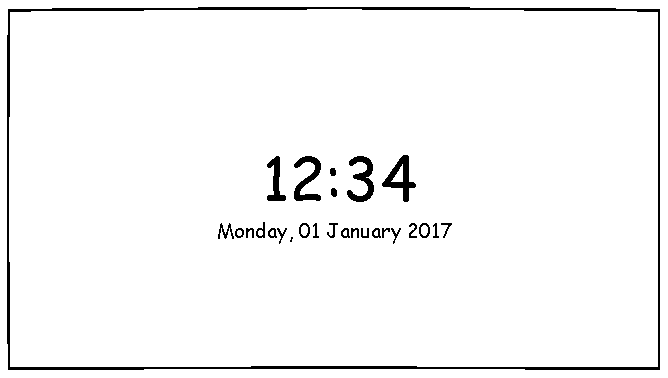
\includegraphics[page=1]{gui-idle}
  \caption{Idle View}
  \label{fig:gui-idle}
\end{figure}

\paragraph{}
The home view (Figure ~\ref{fig:gui-home}) is a basic menu of buttons which allows the user to begin their chosen activity.

\begin{figure}
  \centering
  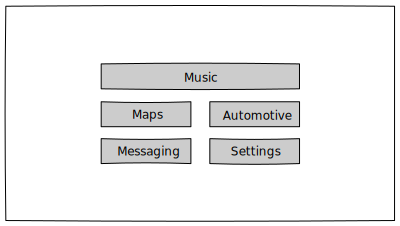
\includegraphics[page=1]{gui-home}
  \caption{Home View}
  \label{fig:gui-home}
\end{figure}

\paragraph{Music Views}
The music views are the primary focus of this project and the most complex.
They mainly synthesize information from the music service to allow navigating a collection of media on connected devices and managing the playback of media.
These views were designed and developed with a focus on minimal amount of interaction with the user in order to minimize distractions.

\begin{figure}
  \centering
  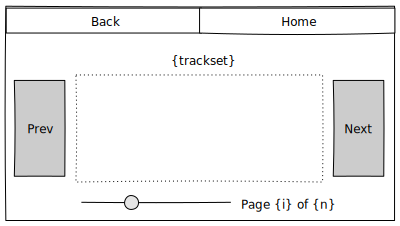
\includegraphics[page=1]{gui-music-trackset}
  \caption{Abstract Track Set Browser}
  \label{fig:gui-music-trackset}
\end{figure}

\paragraph{}
The first music view (Figure ~\ref{fig:gui-music-trackset}) is a abstract browser that is capable of navigating through a single-level list of textual information one page at a time.
This view is realized and slightly refined as an Artists view, an Artist Detail view (Figure ~\ref{fig:gui-music-artist-detail}), an Albums view, Playlists view, an Album view, a Playlist view, and a Track List view.
Each instance of one of these views are stacked on top of each other during navigation and the top view is discarded when the user navigates backward.

\begin{figure}
  \centering
  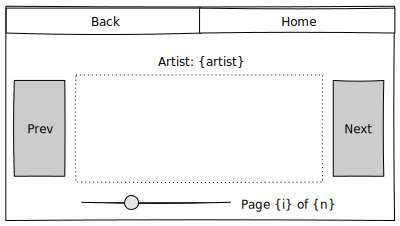
\includegraphics[page=1]{gui-music-artist-detail}
  \caption{Artist Detail View}
  \label{fig:gui-music-artist-detail}
\end{figure}

\paragraph{Maps Views}
When a Geolocation source is available along with mapping data, The GUI contains contain a basic map view, displaying the user's location at a modifiable magnification level.

\paragraph{Messaging Views}
The messaging aspect of the GUI simply display temporary notifications of telephone call as well as text messaging information.
During a hands-free phone call, the user interface view is interrupted to provide call status on the screen.
The messaging subsystem of the GUI is also tasked with implementing the visual side of the Bluetooth device pairing process.

\paragraph{Settings Views}
In order to provide some customizability during runtime, each configurable feature of this project can expose its configurable properties into the application's settings view.
There are also global settings that are configured with this view.
